\subsection{Electrical Power System}

\paragraph{}The electric power system of the satellite must provide and manage the energy generated efficiently in order to have all the systems operating under normal conditions. The Electrical Power System of a Cubesat is, probably, the most fundamental requirement of the satellite payload, since its failure would result in the mission failure. The functions of the EPS are to control and distribute power to the Cubesat, to suppy a continuous source of electrical power for through the lifetime of the mission, to protect the satellite against bus failiures and to monitor and communicate the system status to the on-board computer. The role of the EPS is very diverse and the following subsystems have to be analyzed in detail.

\begin{figure}[h]
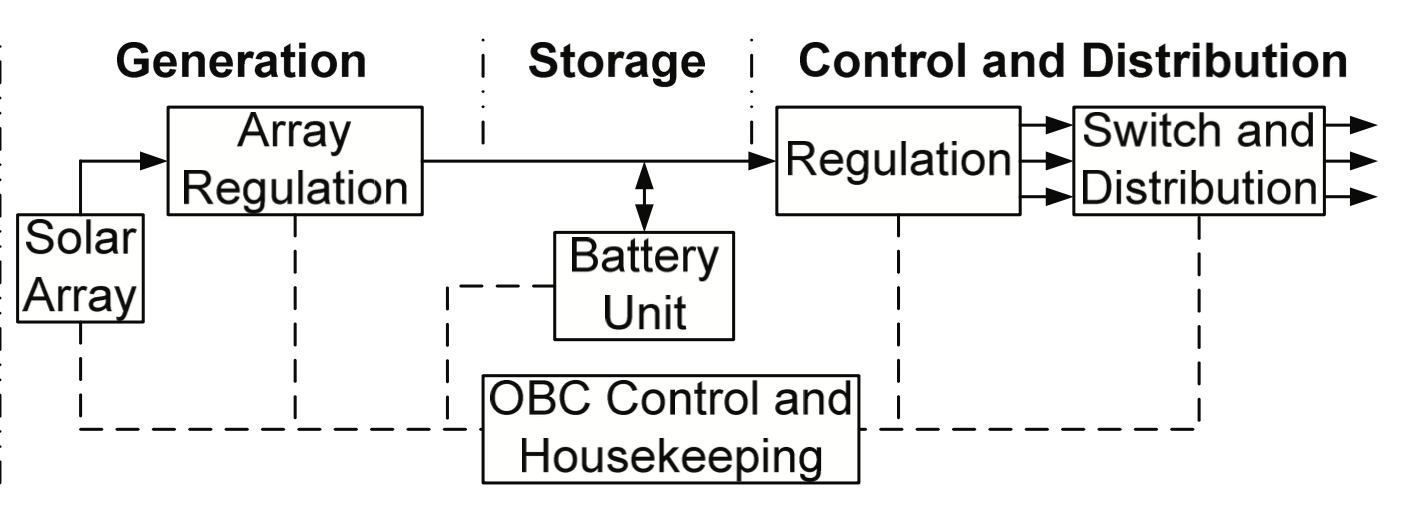
\includegraphics[scale=0.6]{./sections/SatelliteDesign/images/EPSschematics}
\centering
\caption{Basic schematics of the EPS \cite{epsbasics}}
\end{figure}

\subsubsection{Solar arrays}

\paragraph{}The primary source of electrical power has to be photovoltaic cells, given the size of the CubeSat. The photovoltaic cells will collect and convert the energy of the sun into electrical energy. Since they are main power source, they have to be correctly selected to prevent failure. Among the characteristics we seek for our mission, we are looking specially wheter the solar cell has a decent amount of power collection, low mass, protective radiation shield, deployment system, great temperature range and compatibility with the other systems.
\paragraph{}The selected option for the Astrea mission will be a set deployable solar panels provided by EXA (Agencia Espacial Civil Ecuatoriana). These panels are low mass (135g each), have a protective radiation shield (NEMEA Anti Radiation Shield protects the solar panels of EM, High Gamma, X-Ray, Alfa, Beta and low neutron radiation), a very high temperature range (from -80 to 130ºC), a gentle release and deployment with artificial muscles (developed by EXA) and provide a power of 16.8W each (19.2V@0.5A). \\
\paragraph{}Every cubesat will have 4 deployable solar panels providing it with ~67.2W of power to supply peak demands while it is operating. Additionally, it is worth mentioning that these solar arrays are compatible with the hardwared used in each of the satellites.

\subsubsection{Power management}

\paragraph{}The role of the power management systems is to distribute the power and supply the energy to the different systems used in the CubeSat.

\subsubsection{Batteries}

\paragraph{}	Batteries are essential for a proper mission operation. They will provide the spacecraft subsystems with the power needed when the solar arrays are working less efficiently or not properly. Astrea is looking for decent capacity batteries that provide a slightly high typical energy and power, since the subsystems will not usually operate under peak conditions.
\paragraph{}Through the lifetime of the mission, the solar arrays will face an important unfavorable condition; in the worst case scenario, the satellite will be in the dark during half of the time of the orbit. Thus, the batteries must store and supply the energy needed for this time.

\paragraph{}Among all the commercial options, Astrea has chosen the \textit{NanoPower BP4} batteries. The CubeSat will have two of these batteries, with a total capacity of 20800mAh or 77Wh. Each battery has a total of 4 cells, highly stackable and come with a temperature sensor and a heater that will automatically turn on if the temperature is worsening the whole operation of the system. 

\subsubsection{Study of the commercial available options}
\paragraph{}A broad marked study is needed since all the options have to be considered. For this reason, and with the aim to show all the information and features of each system that has been considered in this section, the table \ref{epsoptions} is presented below.

\begin{longtable}{| l | c | c | }
\hline
\rowcolor[gray]{0.80}	\textbf{Brand and model} &  \textbf{Features}     & \textbf{Total price (\euro)}   \\
\hline
\endfirsthead

\rowcolor[gray]{0.85} \textbf{Structure} &  &  \\
	   ~EXA-Agencia Espacial Ecuatoriana & \makecell{Total power of 67.2W (4units)\\ Mass of 270g (p.unit) \\ Included thermal protection \\At least 4 years lifetime} & 17000 \\
	   \hline
	   ~ISIS & \makecell{Total ower of ~30W (4units) \\ Mass of 150g (p.unit) \\ No thermal protection \\At least 2 years lifetime} & \textbf{TO REQUEST!} \\
	   \hline
\rowcolor[gray]{0.85} \textbf{Batteries} &  &  \\
	   ~Gomspace NanoPower BP4 & \makecell{Total capacity of 77Wh \\ Automatic heat regulation \\ Highly stackable \\ Mass of 270g (p.unit)} & \textbf{TO REQUEST!} \\
	\hline
	~EXA-Agencia Espacial Ecuatoriana & \makecell{Total capacity of 53.2Wh \\ Automatic heat regulation \\ Highly stackable \\ Total mass of 155g} & 6300 \\
	\hline
	
\caption{Options studied}
\label{epsoptions}
\end{longtable}

\paragraph{}Finally, the options chosen are presented in the table \ref{epsfinal}.

\begin{longtable}{| l | r | r | }
\hline
\rowcolor[gray]{0.80}	\textbf{System} &  \textbf{Brand and model}     & \textbf{Price per unit (\euro)}   \\
\hline
\endfirsthead

	   ~Solar arrays & EXA-Agencia Espacial Civil Ecuatoriana & 17000 \\
	   ~Batteries & Gomspace, Nanopower BP4 & \textbf{TO REQUEST!} \\
	   ~Power Management & Gomspace, Nanopower & \textbf{TO REQUEST!} \\
	\hline

\caption{Options studied}
\label{epsfinal}
\end{longtable}